% !TeX spellcheck = en_GB
\section{Instruments} \label{sec:DIM}


Many factors such as humidity and temperature contribute to snowflake geometry. The knowledge of snowflake habits, particle size distributions, and fall speed lead to a reduction of errors in optimal estimation retrievals. \\
This work is based on several datasets collected at the Haukeliseter measurement site, \ang{59.8}\,N, \ang{7.2}\,E. A composition of advanced ground-based observations and the CloudSat precipitation retrieval will help to get a better understanding of the vertical structure of the atmosphere. 
\\
%%%%%%%%%%%%%%%%%%%%%%%%%%%%%%%%%%%%%%%%%%%%%%%%%%%%%%%%%%%%%%%%%%%%%%%%%%
%%%%%%%%%%%%%%%%%%%%%%%%%%%%%%%%%%%%%%%%%%%%%%%%%%%%%%%%%%%%%%%%%%%%%%%%%%
%%%%%%%%% INTSTRUMENTS %%%%%%%%%%%%%%
%\section{Instruments}\label{sec:instruments}
A collaboration between the University of Utah, University of Wisconsin and Met-Norway made it possible to install three additional instruments at the measurement site during winter 2016/2017. A Multi-Angle Snowflake Camera (MASC) and a Precipitation Imaging Package (PiP) will be used to determine the snow habit, the snowfall particle size distribution, and near-surface fall speed. Additionally, a Micro Rain Radar (MRR) is established to obtain fall speed and particle reflectivity aloft. Together with temperature observations at the surface, is this a good basis to reduce the non-uniqueness of snow accumulation in optimal estimation snowfall retrieval, described in \Cref{sec:retrieval}. 
%%% image instrument setting @ Haukeli %%%%%%%%%%%%%%%%%%%%%%%%%%%%%%%%%%%%%
% !TeX spellcheck = en_GB

\begin{figure}
\centering
	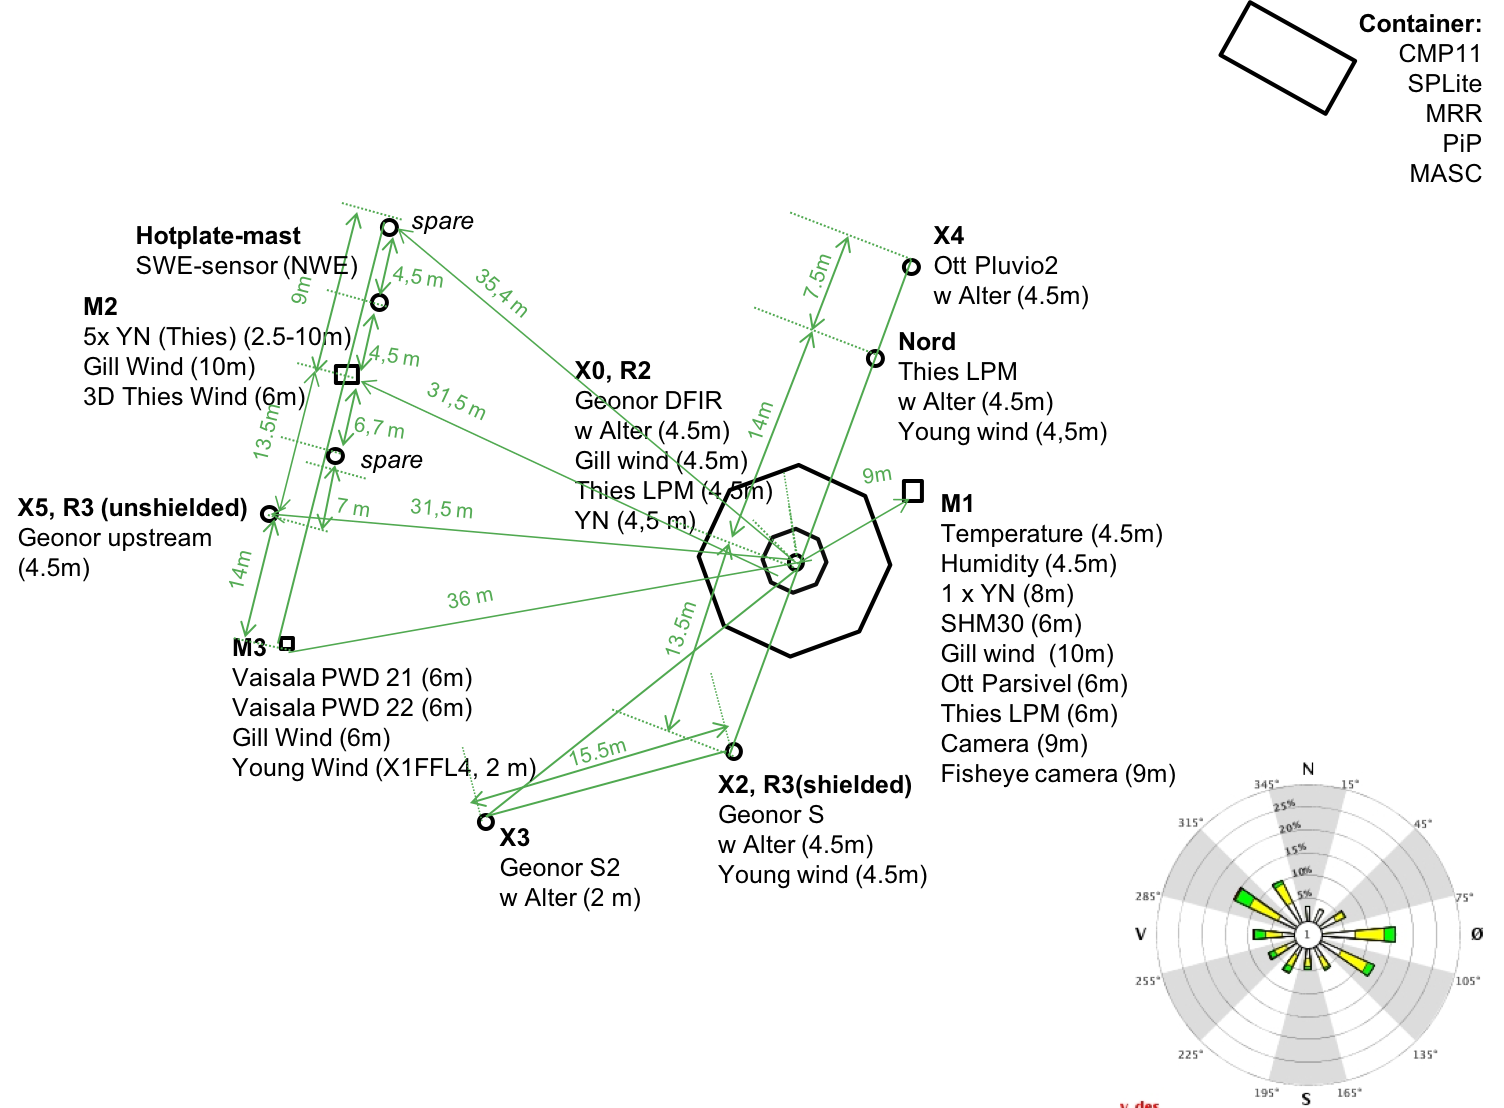
\includegraphics[width=\textwidth]{./fig_instruments/instrument_setting.png}
	%	\vspace{-10pt}
	\caption{Instruments at the Haukeliseter measurement site during winter 2016/2017 \citep[adapdet from][]{wolff_derivation_2015}. The windrose indicates the mean wind direction from either from west-north-west or east-south-east.}\label{fig:inst_setting}
\end{figure}

%%%%%%%%%%%%%%%%%%%%%%%%%%%%%%%%%%%%%%%%%%%%%%%%%%%%%%%%%%%%%%%%%%%%%%%%%%
\noindent
A sketch of the instrumentation setting is presented in \Cref{fig:inst_setting}. The octagonal indicates the double fence. The container is north-east from the double fence having the MRR, MASC and PiP mounted at the top. \textbf{M1} in \Cref{fig:inst_setting} is the \SI{10}{\metre} weather mast, providing the hourly \citet{eklima_norwegian_2016} temperature, pressure, and wind measurements. The mean wind direction from west-north-west and east-south-east are shown in the wind rose in \Cref{fig:inst_setting}.
%
%
%\pagebreak
%%%%%%%%%%%%%%%%%%%%%%%%%%%%%%%%%%%%%%%%%%%%%%%%%%%%%%%%%%%%%%%%%%%%%%%%%%
%%%%%%%%%%%%%%%%%%%%%%%%%%%%%%%%%%%%%%%%%%%%%%%%%%%%%%%%%%%%%%%%%%%%%%%%%%
%%%%%%%%% DOUBLE FENCE %%%%%%%%%%%%%%
\subsection{Double Fence}\label{sec:dofe}
%%% image double fence @ Haukeli %%%%%%%%%%%%%%%%%%%%%%%%%%%%%%%%%%%%%
% !TeX spellcheck = en_GB
% \begin{figure}[h!]
% 	\centering
% 		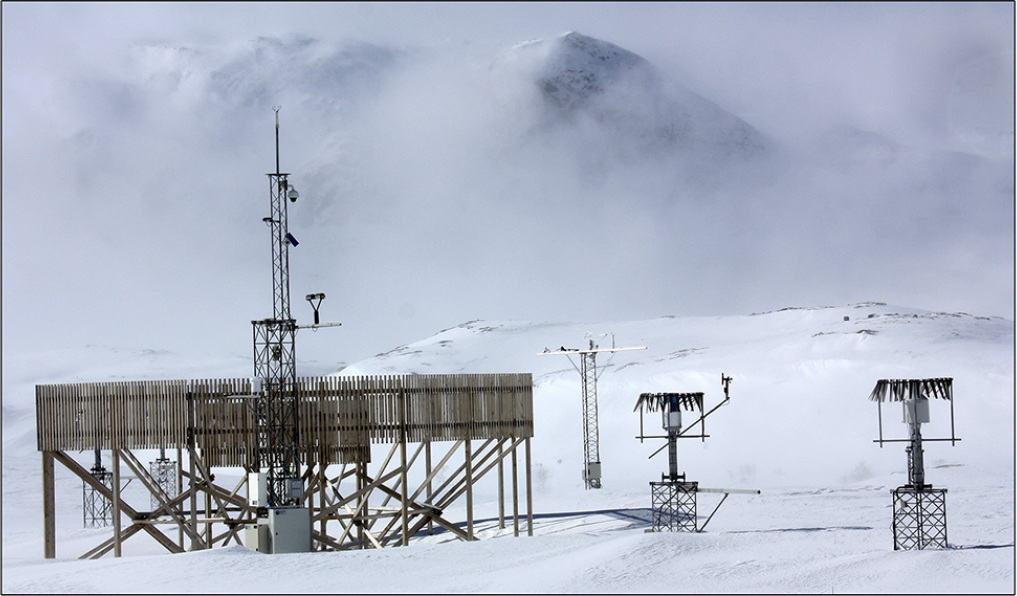
\includegraphics[width=0.55\textwidth]{./fig_instruments/Dofe.png}
% 	\caption{Picture, showing the double fence and unprotected precipitation gauges at the measurement site Haukeliseter. Picture taken from \cite{wolff_derivation_2015}.}\label{fig:Dofe}
% \end{figure}



\begin{wrapfigure}[28]{r}{0.44\textwidth}
	\vspace{-\normalbaselineskip}
	\centering
	\begin{subfigure}[b]{0.4\textwidth}
		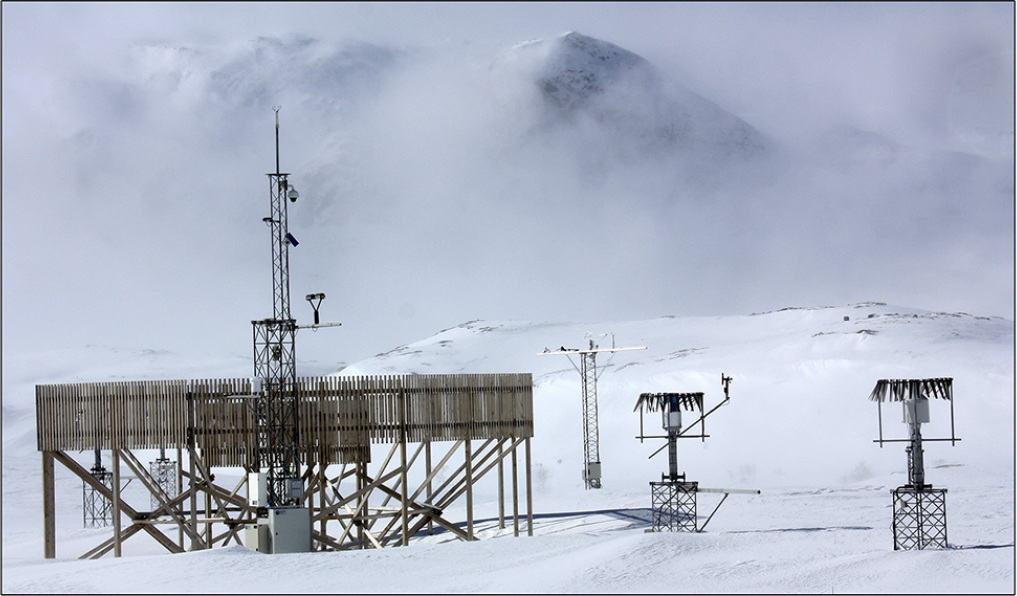
\includegraphics[width=\textwidth]{./fig_instruments/Dofe.png}
		\caption{}\label{fig:dofe_pic}
	\end{subfigure}	
	\begin{subfigure}[b]{0.4\textwidth}
		% 		\includegraphics[trim={0.8cm, 2.3cm, 2.4cm, 3cm},clip,width=1.1\textwidth]
		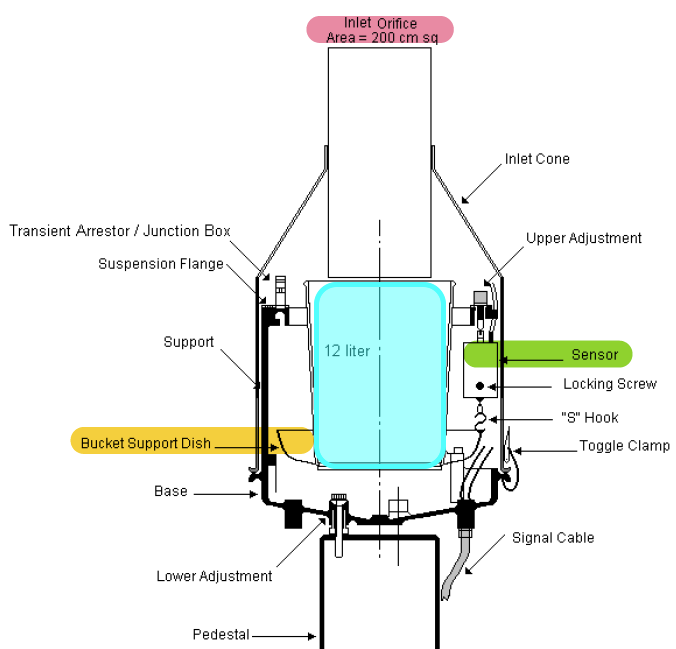
\includegraphics[width=1.1\textwidth]{./fig_instruments/Geonor_sketch2.png}
		\caption{}\label{fig:gauge_sketch}
	\end{subfigure}	
	\caption{(\protect\subref{fig:dofe_pic}) From left to right: Double fence gauge (\textbf{X0}) and unprotected precipitation gauges (\textbf{Nord, X4}) at Haukeliseter, from \cite{wolff_derivation_2015}. The prevailing easterly (westerly) wind from the lower, left corner in \protect\subref{fig:dofe_pic} (the opposite site). In front of the double fence gauge is the \SI{10}{\metre} weather mast (\textbf{M1}). (\protect\subref{fig:gauge_sketch}) Vertical cross section of Geonor T-200B3 precipitation gauge. pink: orifice; cyan: cylindric bucket with frost protection; yellow: bucket support dish; green: wire sensor \citep[adapted from][]{geonor_inc._t-200b_2015}.  }\label{fig:Dofe}
	%	\vspace{-\normalbaselineskip}
\end{wrapfigure}
%%%%%%%%%%%%%%%%%%%%%%%%%%%%%%%%%%%%%%%%%%%%%%%%%%%%%%%%%%%%%%%%%%%%%%%%%%
Since the winter season 2010/2011 Haukeliseter is equipped with several precipitation gauges. The wind shielded gauges are placed perpendicular to the main wind direction (E/W wind).
\\
In a study by \citet{wolff_derivation_2015} the wind-induced under-catch of solid precipitation is determined. Dependent on the kind of precipitation the wind plays different roles in the amount of accumulation. For temperatures below \SI{-2}{\celsius} the wind speed influences the falling snow. Where less precipitation can be observed at higher wind speeds or more precipitation can be measured if too much is blown into the gauge. The catch ratio between the standard Geonor precipitation gauge and the Double Fence - Geonor (\Cref{fig:dofe_pic}) shows, that only \SI{80}{\percent} of solid precipitation are observed at wind speeds of \SI{2}{\mPs} and only \SI{40}{\percent} at \SI{5}{\mPs}, \citet[Figure 5 in][]{wolff_derivation_2015}. 
\\
The precipitation gauge protected by an octagonal double fence (\Cref{fig:dofe_pic}) is more accurate than the single fence and will be used as the reference to all surface accumulation measurements. The double fence creates an artificial calm wind and maximize the catch of precipitation, \citep{wolff_new_2010, wolff_measurements_2013, wolff_derivation_2015}. The wind inside the double fence is measured to be not much higher than \SI{5}{\mPs} even if the winds outside exceed \SI{20}{\mPs} (occurred \SI{26}{\dec}). % so far it is unknown, if the catch efficiency stabilises for wind speeds beyond \SI{10}{\mPs} and may lead to wrong values
\\
This shows the need of a combination of ground-based observations together with an optimal estimation retrieval to verify the accuracy of MEPS. \citet{wolff_derivation_2015} introduced an adjustment function for the Geonor double fence, so that different precipitation under certain wind speeds are presented correctly and can be used as confidential data. 
For now, it is presumed that the average under catch inside a double fence is \SI{20}{\percent} for wind speeds between \SIlist{10;20}{\mPs} and \SI{10}{\percent} for wind speeds under \SI{9}{\mPs} \citep{wolff_wmo_2018}.
\\ \\
Inside the double fence is a precipitation-weighing gauge Geonor T-200B3 \citep[3-wire transducers, \SI{1000}{\mm},][]{geonor_inc._t-200b_2015} with an Alter wind screen to reduce wind turbulence around the gauge. At Haukeliseter is the orifice height of the Geonor \SI{4.5}{\metre} above the ground. This is due to an expected snow depth of \SIrange{2}{3}{\metre} during a winter season and to reduce the likelihood of measuring drifting snow \citep{wolff_measurements_2013,wolff_derivation_2015}. \\
A vertical cross section of the T-200B gauge is shown in \Cref{fig:gauge_sketch}. Precipitation particles fall through the \SI{200}{\square\cm} orifice protected with a heated collar, into a cylindric bucket filled with frost protection. The bucket is placed on top of a Bucket Support Dish \citep[\Cref{fig:gauge_sketch},][]{geonor_inc._t-200b_2015}. This dish is connected with three wire sensors having an eigenfrequency changing with the weight inside the bucket. A formula provided by \citet{geonor_inc._t-200b_2015} calculates the amount of precipitation from the frequency of each sensor. The three sensors provide a reduction of an error in connection with an unlevel installation. Met-Norway will average value of all three sensors and provide it as hourly data at \citeauthor{eklima_norwegian_2016}.
%%%%%%%%%%%%%%%%%%%%%%%%%%%%%%%%%%%%%%%%%%%%%%%%%%%%%%%%%%%%%%%%%%%%%%%%%%
%%%%%%%%%%%%%%%%%%%%%%%%%%%%%%%%%%%%%%%%%%%%%%%%%%%%%%%%%%%%%%%%%%%%%%%%%%
%%%%%%%%% MRR %%%%%%%%%%%%%%
\subsection{MRR - Micro Rain Radar}\label{sec:MRR}
%%% image MRR instrument %%%%%%%%%%%%%%%%%%%%%%%%%%%%%%%%%%%%%
% !TeX spellcheck = en_GB
% \begin{figure}[h!]
% 	\centering
% 		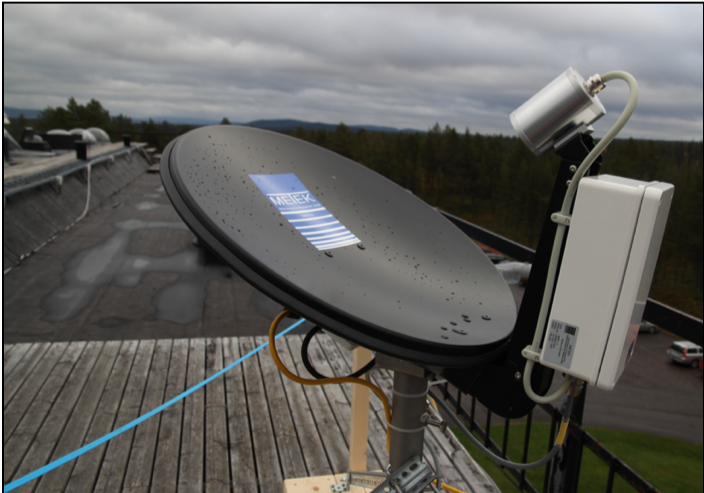
\includegraphics[width=0.55\textwidth]{./fig_instruments/MRR.png}
% 	\caption{MRR from METEK}\label{fig:MRR}
% \end{figure}

\begin{wrapfigure}[14]{r}{0.44\textwidth}
	\vspace{-\normalbaselineskip}
	\centering
	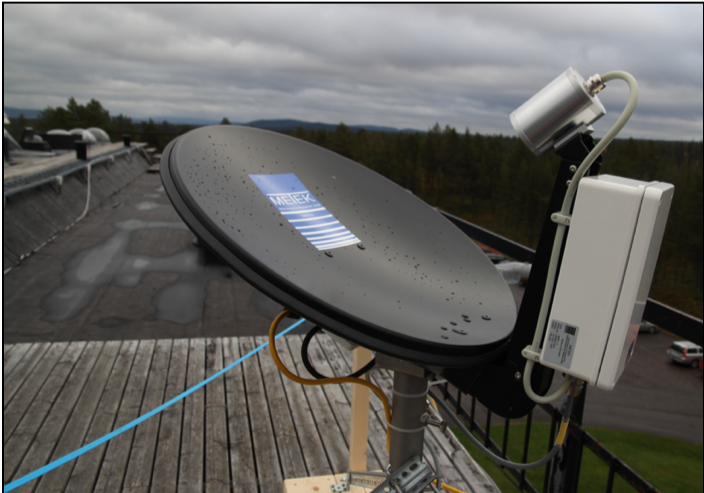
\includegraphics[width=0.4\textwidth]{./fig_instruments/MRR.png}
	%	\vspace{-10pt}
	\caption{Micro Rain Radar at the measurement site in Kiruna. Transceiver transmits Radar signal using the antenna (parabolic dish) and receives backscatter signal over the antenna. During winter 2016/2017 installed at Haukeliseter (\textbf{container}).}\label{fig:MRR}
	\vspace{-\normalbaselineskip}
\end{wrapfigure}
%%%%%%%%%%%%%%%%%%%%%%%%%%%%%%%%%%%%%%%%%%%%%%%%%%%%%%%%%%%%%%%%%%%%%%%%%%
Radars are very useful to observe the vertical of the atmosphere. The instrument is able to detect mesoscale features and makes it possible to see the vertical structure of storms \citep{markowski_mesoscale_2011}.\\
The principle of radar measurements is based on an electromagnetic wave, which is emitted from the radar transmitter and interacts with the hydrometeors along the beam. A fraction of the pulse energy is reflected back to the receiver of the radar. The quantity of scattering depends on the shape and structure of the reflected particle. 
Vertical profiles of reflectivity give information about the diameter of the target object.
\\
The Micro Rain Radar, in \Cref{fig:MRR}, measures profiles of Doppler spectra \citep{metek_micro_2010}. The Doppler spectrum tells about the movement of the particle. The vertical pointing Doppler radar measures the energy that is returned from each interval and thus enabling the detection of the Doppler spectrum \citep{lecuyer_aos_2017}. The MRR measures at a frequency of \SI{24}{\giga\Hz} and has a temporal and spatial resolution of \SI{60}{\second} and \SI{100}{\metre}, respectively. The radar height range is from \SI{100}{\metre} (because of ground clutter) to \SI{3.000}{\metre} \citep{metek_micro_2010}.
\\
MRR radar reflectivity ($Z$) is transformed from \SI{1}{\mm^6\per\metre^3} to \SI{}{\decibel\,Z}.
The transformations are done with the following relationship;
\begin{align}
	Ze & = 10 \log_{10} \left(\frac{Z}{\SI{1}{\mm^6\per\metre^3}}\right) \qquad [\SI{}{\decibel Z}]
	\label{eq:Ze}
\end{align}
A transformation to rainfall rates can be performed by the $Z$-$R$ (reflectivity - rainfall) relationship. 
The rainfall rate in each layer can be estimated by the use of typical fall speeds and the Marshall-Palmer particle size distribution for liquid particles \citep{rinehart_radar_2010}. 
\begin{align}
	Z & = 200 R^{\frac{8}{5}} \qquad [\SI{}{\mm^6\metre^{-3}} ] \nonumber \\ 
	R & = \left( \frac{ 10^{\frac{Ze}{10}} }{200} \right)^{\frac{8}{5}} \qquad [ \SI{}{\mm\per\hour} ]
	\label{eq:Z-R}
\end{align}
\\
\Cref{tab:ref_values} represents the Z-R relationship if the Marshall-Palmer assumption (\Cref{eq:Z-R}) is applied. Z-snowfall relationships are developed but are difficult to apply due to the variation of size and density of the particles \citep{lecuyer_aos_2017}. \\
After the transformation to \SI{}{\decibel Z} the reflectivity is averaged for every \SI{200}{\metre} layer thickness, where only values above \SI{300}{\metre} are taken. 
For instance, a reflectivity at \SI{400}{\metre} represents the mean value of reflectivity between \SIlist{300;500}{\metre}. 
%%% table REFLECTIVITY AND RAINRATE %%%%%%%%%%%%%%%%%%%%%%%%%%%%%%%%%%%%%
% % !TeX spellcheck = en_GB
\begin{table}[t]
	\begin{center}
		\caption{Typical reflectivity values, from \cite{doviak_doppler_1993}. The values are obtained from measurements, models and observations. The rainfall rate $R$ is calculated with \Cref{eq:Z-R}. }\label{tab:ref_values}
		\begin{tabular}{ll|c|c}
			\hline \hline
			\multicolumn{2}{l|}{} & \textbf{Ze} & \textbf{R} \\ 
			\multicolumn{2}{l|}{} & [\SI{}{\decibel Z}] & [\SI{}{\mm\per\hour}] \\ \hline \hline
			\multicolumn{2}{l|}{\textbf{Drizzle}} & \num{< 25} &  \num{1.3} \\ \hline
			\multicolumn{2}{l|}{\textbf{Rain}} & \numrange{25}{60} & \numrange{1.3}{205.0} \\ \hline
			\multicolumn{2}{l|}{\textbf{Snow}} &  \\ 
			& dry, low density 	& \num{< 35} & \num{5.6}\\ \hline
			& Crystal; dry, high density & \num{< 25} & \num{1.3}\\ \hline
			& wet, melting 		& \num{< 45} & \num{23.7} \\ \hline
			\multicolumn{2}{l|}{\textbf{Graupel}} & \\
			& dry 				& \numrange{40}{50} & \numrange{11.5}{48.6} \\ \hline
			& wet				& \numrange{40}{55} & \numrange{11.5}{99.9} \\ \hline
			\multicolumn{2}{l|}{\textbf{Hail}} & \\
			& small; \SI{< 2}{\cm}, wet & \numrange{50}{60} & \numrange{48.6}{205.0}\\
			& large; \SI{> 2}{\cm}, wet & \numrange{55}{70} & \numrange{99.9}{864.7}\\ \hline
			\multicolumn{2}{l|}{\textbf{Rain \& Hail}} & \numrange{50}{70} & \numrange{48.6}{864.7} \\ 
			\hline \hline
		\end{tabular}
	\end{center}
\end{table}
%%%%%%%%%%%%%%%%%%%%%%%%%%%%%%%%%%%%%%%%%%%%%%%%%%%%%%%%%%%%%%%%%%%%%%%%%%

\newpage
%%%%%%%%%%%%%%%%%%%%%%%%%%%%%%%%%%%%%%%%%%%%%%%%%%%%%%%%%%%%%%%%%%%%%%%%%%
%%%%%%%%%%%%%%%%%%%%%%%%%%%%%%%%%%%%%%%%%%%%%%%%%%%%%%%%%%%%%%%%%%%%%%%%%%
%%%%%%%%% PiP %%%%%%%%%%%%%%
\subsection{PiP - Precipitation Imaging Package}
%%% image PiP instrument %%%%%%%%%%%%%%%%%%%%%%%%%%%%%%%%%%%%%
% !TeX spellcheck = en_GB
% \begin{figure}[h!]
% 	\centering
% 		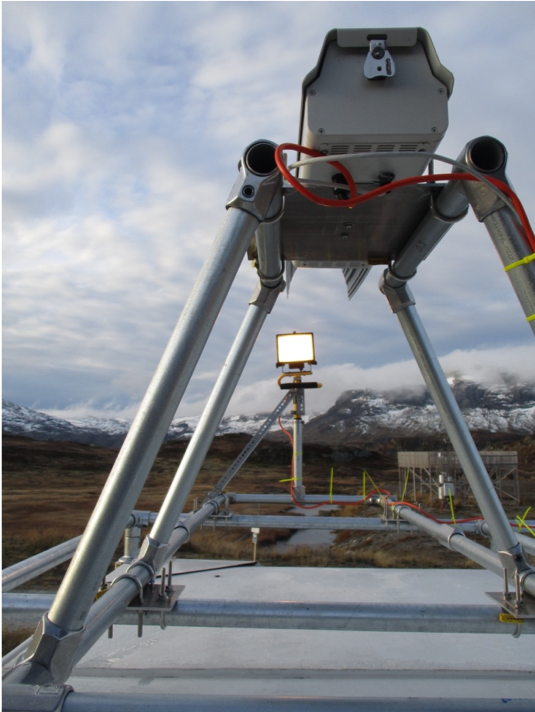
\includegraphics[width=0.35\textwidth]{./fig_instruments/PiP.png}
% 	\caption{PiP}\label{fig:PiP}
% \end{figure}

\begin{wrapfigure}[21]{r}{0.44\textwidth}
	\vspace{-\normalbaselineskip}
	\centering
	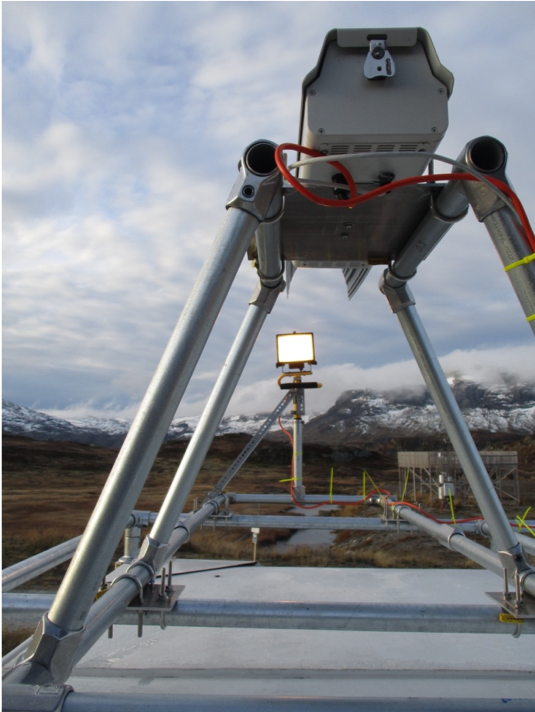
\includegraphics[trim={3.cm, 3.3cm, .5cm, 0cm},clip,width=0.4\textwidth]{./fig_instruments/PiP.png}
	%	\vspace{-10pt}
	\caption{Precipitation Imaging Package at Haukeliseter mounted at the \textbf{container} pointing towards the double fence gauge.}\label{fig:PiP}
	\vspace{-\normalbaselineskip}
\end{wrapfigure}
%%%%%%%%%%%%%%%%%%%%%%%%%%%%%%%%%%%%%%%%%%%%%%%%%%%%%%%%%%%%%%%%%%%%%%%%%%
The precipitation imaging package (PiP) is a modification of the Snowflake Video Imager presented by \citet{newman_presenting_2009}. The video distrometer is a construct of a halogen flood lamp and a video system (\Cref{fig:PiP}). The instrument determines the habit of snowflakes from images at a frequency of \SI{60}{\Hz}. Lamp and lens have a distance of approximately \SI{3}{\metre} which follows a field of view: \SI{32}{\mm} by \SI{24}{\mm}. 
\\
In front of the halogen lamp is a frosted window, so that the background light is uniform over all time. A falling particle appears as a 2-D shadow in the video image. 
Particle size distribution (PSD) and fall speed of precipitation can be determined from the black and white images of the system.
\citet{newman_presenting_2009} describes in detail the algorithm applied to the system to get information about the snow-particle habit. \\
Winds have almost no effect on the result of the video distrometer \citep{newman_presenting_2009}. To reduce eventual wind effects, was the distrometer oriented perpendicular to the mean wind.
\newpage
%%%%%%%%%%%%%%%%%%%%%%%%%%%%%%%%%%%%%%%%%%%%%%%%%%%%%%%%%%%%%%%%%%%%%%%%%%
%%%%%%%%%%%%%%%%%%%%%%%%%%%%%%%%%%%%%%%%%%%%%%%%%%%%%%%%%%%%%%%%%%%%%%%%%%
%%%%%%%%% MASC %%%%%%%%%%%%%%
\subsection{MASC - Multi-Angular Snowfall Camera}
%%% image MASC %%%%%%%%%%%%%%%%%%%%%%%%%%%%%%%%%%%%%
% !TeX spellcheck = en_GB
% \begin{figure}[h!]
% 	\centering
% 	\begin{subfigure}[b]{0.55\textwidth}
% 		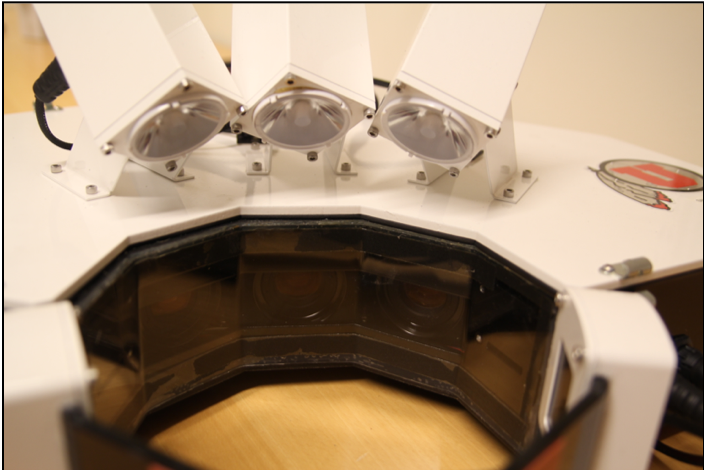
\includegraphics[width=\textwidth]{./fig_instruments/MASC.png}
% 	\end{subfigure}
% 	\begin{subfigure}[b]{0.55\textwidth}
% 		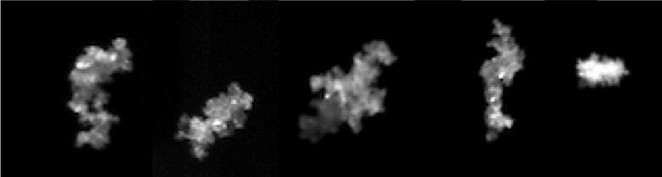
\includegraphics[width=\textwidth]{./fig_instruments/MASC_snowflakes.png}
% 	\end{subfigure}
% 	\caption{Instrument MASC, and images taken by the instrument. \textcolor{red}{lower panel taken from \cite{cooper_variational_2017} maybe we get one for Haukeli?}}\label{fig:MASC}
% \end{figure}

% \begin{wrapfigure}[17]{r}{0.44\textwidth}
\begin{wrapfigure}[15]{r}{0.44\textwidth}
	\vspace{-\normalbaselineskip}
	\centering
	\begin{subfigure}[b]{0.4\textwidth}
		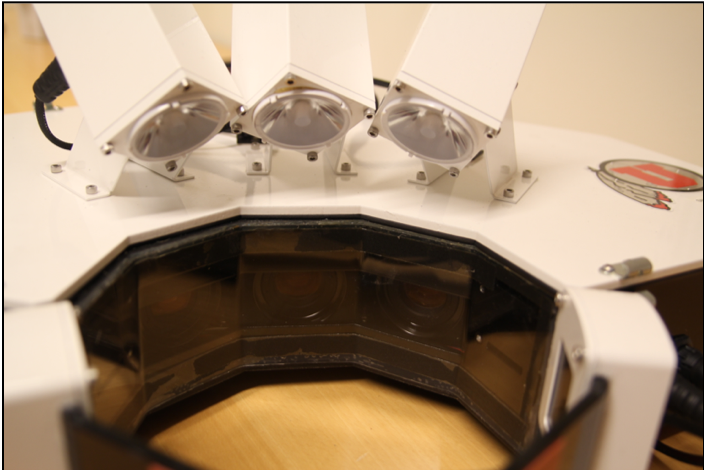
\includegraphics[trim={1.cm, 0cm, .8cm, 0cm},clip,width=\textwidth]{./fig_instruments/MASC.png}
	\end{subfigure}	
	\begin{subfigure}[b]{0.4\textwidth}
		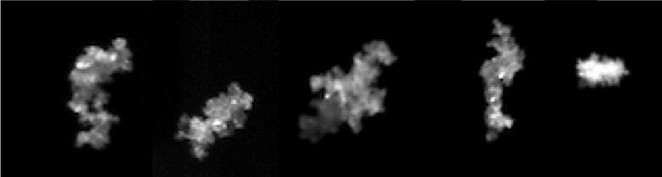
\includegraphics[width=\textwidth]{./fig_instruments/MASC_snowflakes.png}
	\end{subfigure}	
	\caption{Multi-Angular Snowfall Camera and images taken by the instrument during the Christmas storm 2016. Located on \textbf{container}.}\label{fig:MASC}
	%	\vspace{-\normalbaselineskip}
\end{wrapfigure}
%%%%%%%%%%%%%%%%%%%%%%%%%%%%%%%%%%%%%%%%%%%%%%%%%%%%%%%%%%%%%%%%%%%%%%%%%%
Instruments like the afore mentioned PiP has according to \citet{garrett_fall_2012} coarser resolution and the determination of particle size can have larger errors. Hence, a new instrument was developed. The Multi-Angular Snowfall Camera (MASC) takes high-resolution images of hydrometeors in free fall and measures the fall-speed simultaneously. \\
The MASC consists of three cameras, three flashes, and two near-infrared sensors, pointing at a ring centre (\Cref{fig:MASC}). A hydrometeor has to pass through the ring in a certain way to trigger the near-infrared sensors. At the same time the three cameras take a picture of the falling particle. Since the cameras take pictures from three different angles, the particles size, shape, and orientation can be specified from an algorithm applied to the image, described in \citet{garrett_fall_2012}. Furthermore, the form and heritage of the hydrometeor, such as collision-coalescence, riming, capture nucleation, or aggregation, can be determined. \\
The near-infrared sensor, that is used to trigger the cameras and the lights quantifies the fall-speed of the hydrometeors, by measuring the time the particle needs to pass the distance between the upper and lower trigger.    
